% Created 2021-10-01 Fri 21:46
% Intended LaTeX compiler: pdflatex
\documentclass{article}
\usepackage[utf8]{inputenc}
\usepackage[T1]{fontenc}
\usepackage{graphicx}
\usepackage{grffile}
\usepackage{longtable}
\usepackage{wrapfig}
\usepackage{rotating}
\usepackage[normalem]{ulem}
\usepackage{amsmath}
\usepackage{textcomp}
\usepackage{amssymb}
\usepackage{capt-of}
\usepackage{hyperref}

\usepackage[a4paper,left=0.5in,right=0.5in,top=0.5in,bottom=1in]{geometry}
\usepackage{float}
\usepackage{enumerate}
\DeclareUnicodeCharacter{2212}{-}
\setcounter{secnumdepth}{0}
\author{Tzong Lin Chua}
\date{\today}
\title{EE4C10 Analog Circuit Design Fundamentals\\\medskip
\large Homework Assignment III }
\hypersetup{
 pdfauthor={Tzong Lin Chua},
 pdftitle={EE4C10 Analog Circuit Design Fundamentals},
 pdfkeywords={},
 pdfsubject={},
 pdfcreator={Emacs 27.1 (Org mode 9.5)}, 
 pdflang={English}}
\begin{document}

\maketitle
\tableofcontents


\section{Simulation Files}
\label{sec:org6d3b08f}
Each question with simulation files will have their respective subfolder.
Except for \texttt{q4}, the other questions will have separate subfolders for common-mode and differential mode circuits.

Running the simulation files should be able to directly plot the graphs used (configured in the *.plt file) or the operation points.
The folders for each question are arranged as follows after extracting:

\begin{center}
\begin{tabular}{lll}
\hline
spice &  & \\
 & q3 & \\
 &  & cm\\
 &  & dm\\
 & q4 & \\
 & q5 & \\
 &  & cm\\
 &  & dm\\
\hline
\end{tabular}
\end{center}
\section{Problem 1}
\label{sec:org072a76a}
\begin{enumerate}[(a)]
\item Overdrive voltage of NMOS transistor M1 and M2, V\textsubscript{OV1} and V\textsubscript{OV2}.

Drain current of M1 and M2 for 0 differential input,
\begin{equation*}
\begin{aligned}
I_{D1} = I_{D2} &= \frac{I_{DD}}{2} = 75 \mu{}A \\
\\
I_{D1} &= \frac{\mu_{n}C_{OX}}{2}\frac{W}{L}(V_{OV1})^{2} \\
V_{OV1} &= \sqrt{\frac{2I_{D1}}{\mu_{n}C_{OX}}\frac{L}{W}} \\
&= 0.316 V \\
\\
V_{OV1} = V_{OV2} &= 0.316V \\
\end{aligned}
\end{equation*}

\item \(\Delta{}I_{D}\) when \(\Delta{}V_{in}\)
\begin{equation*}
\begin{aligned}
I_{D1} &= \frac{\mu_{n}C_{OX}}{2}\frac{W}{L}(V_{OV1} + \frac{\Delta{}V_{in}}{2})^{2} \\
&= 82.28 \mu{}A \\
\Delta{}I_{D1} &= I_{D1} - \frac{I_{DD}}{2} \\
&= 7.28 \mu{}A \\
\\
I_{D2} &= \frac{\mu_{n}C_{OX}}{2}\frac{W}{L}(V_{OV2} - \frac{\Delta{}V_{in}}{2})^{2} \\
&= 68.05 \mu{}A \\
\Delta{}I_{D2} &= I_{D2} - \frac{I_{DD}}{2} \\
&= -6.95 \mu{}A \\
\Delta{}I_{D} &= \Delta{}I_{D1} + \Delta{}I_{D2} \\
&= 14.23 \mu{}A \\
\end{aligned}
\end{equation*}

\item Equivalent g\textsubscript{m}.

Since M1 and M2 has the same dimensions,
\begin{equation*}
\begin{aligned}
g_{m} &= 2g_{m1} = 2g_{m2} \\
&= 2\frac{\mu_{n}C_{OX}}{2}\frac{W}{L}V_{OV1} \\
&= 474 \mu{}S \\
\end{aligned}
\end{equation*}
\end{enumerate}

\section{Problem 2}
\label{sec:org574b9e5}
\begin{enumerate}[(a)]
\item \(I_{b}\) when \(I_{D2} = I_{D3} = 0.8(\frac{I_{SS}}{2})\)
\begin{equation*}
\begin{aligned}
I_{D2} = I_{D3} &= 0.8 \frac{I_{SS}}{2} \\
&= 0.4 mA \\
\\
I_{D1} = I_{D4} &= 0.2 \frac{I_{SS}}{2} \\
&= 0.1 mA \\
\\
\end{aligned}
\end{equation*}
Since transistor M5-M1 and M5-M4 are current mirror pairs,
\begin{equation*}
\begin{aligned}
I_{b} &= I_{D5} = I_{D1} = I_{D4} \\
I_{b} &= 0.1 mA \\
\end{aligned}
\end{equation*}
\item Voltage gain, A\textsubscript{DM-DM}, is equal to the gain of the half circuit.
\begin{equation*}
\begin{aligned}
G_{m} &= g_{m6} \\
\\
R_{out} &= \frac{1}{g_{m2} + \frac{1}{r_{o1}} + \frac{1}{r_{o2}} + \frac{1}{r_{o6}}} \\
\\
A_{DM-DM} &= -G_{m}R_{out} \\
&= \frac{g_{m6}}{g_{m2} + \frac{1}{r_{o1}} + \frac{1}{r_{o2}} + \frac{1}{r_{o6}}} \\
\\
g_{m2} &\approx \sqrt{2\mu_{p}C_{OX}\frac{W}{L}I_{D2}} \\
&\approx 1.342 mS \\
\\
g_{m6} &\approx \sqrt{2\mu_{n}C_{OX}\frac{W}{L}\frac{I_{SS}}{2}} \\
&\approx 2.121 mS \\
\\
r_{o1} &= \frac{1}{I_{D1}\lambda} \\
&= 100 k\Omega \\
r_{o2} &= \frac{1}{I_{D2}\lambda} \\
&= 25 k\Omega \\
r_{o6} &= \frac{1}{I_{D6}\lambda} \\
&= 20 k\Omega \\
\\
A_{DM-DM} &= -1.471 \\
\end{aligned}
\end{equation*}
\item The circuit's:
\begin{enumerate}[1.]
\item CM-CM gain

From the lecture slides,
\begin{equation*}
\begin{aligned}
A_{CM-CM} &= \frac{2g_{m}\frac{r_{o}}{2}\frac{R_{D}}{2}}{\frac{r_{o}}{2}(1 + 2g_{m}R_{SS}) + R_{SS}+\frac{R_{D}}{2}} \\
\\
g_{m} &= g_{m6} \\
&= 2.121mS \\
\\
r_{o} &= r_{o6} \\
&= 20k\Omega \\
\\
R_{D} &= \frac{r_{o1}r_{o2}}{g_{m2}r_{o1}r_{o2} + r_{o1} + r_{o2}} \\
&= 718.4\Omega \\
\\
R_{out} &= \frac{1}{2g_{m2} + \frac{2}{r_{o1}} + \frac{2}{r_{o2}} + \frac{2}{r_{o6}}} \\
\\
A_{CM-CM} &= -\frac{15237}{10359 + 43.42R_{SS}} \\
\end{aligned}
\end{equation*}
Since resistance of ideal current source is infinite, \(A_{CM-CM} = 0\).
\item DM-CM gain

Since the ideal case is considered, there will be no mismatch in resistance or transconductance
\(A_{DM-CM} = 0\)
\item CM-DM gain

Since the ideal case is considered, there will be no mismatch in resistance or transconductance
\(A_{DM-CM} = 0\)

\item CMRR
\begin{equation*}
\begin{aligned}
CMRR &= |\frac{A_{DM-DM}}{A_{CM-DM}}| \\
CMRR &= \infty
\end{aligned}
\end{equation*}
\end{enumerate}

\item Input common-mode range to keep all transistors in saturation.

Range of V\textsubscript{out},
\begin{equation*}
\begin{aligned}
V_{dd} - V_{out} &\geq 0.7 V \\
V_{out} &\leq 1.1 V \\
\end{aligned}
\end{equation*}
Range of V\textsubscript{in},
\begin{equation*}
\begin{aligned}
V_{out} - 0.4V &\geq V_{in} - 0.4 V - 0.7 V\\
V_{in} \leq 1.8 V \\
\\
V_{in} - 0.4 V &\geq 0.7 V \\
V_{in} &\geq 1.1 V \\
\\
1.1 V \leq &V_{in} \leq 1.8 V \\
\end{aligned}
\end{equation*}
\end{enumerate}


\section{Problem 3}
\label{sec:org8c35992}
\begin{enumerate}[(a)]
\item Low frequency
\begin{enumerate}[1.]
\item Differential gain

From figure \ref{fig:dm-q3}, \(A_{DM} = 42.0 dB\)
\begin{figure}[H]
\centering
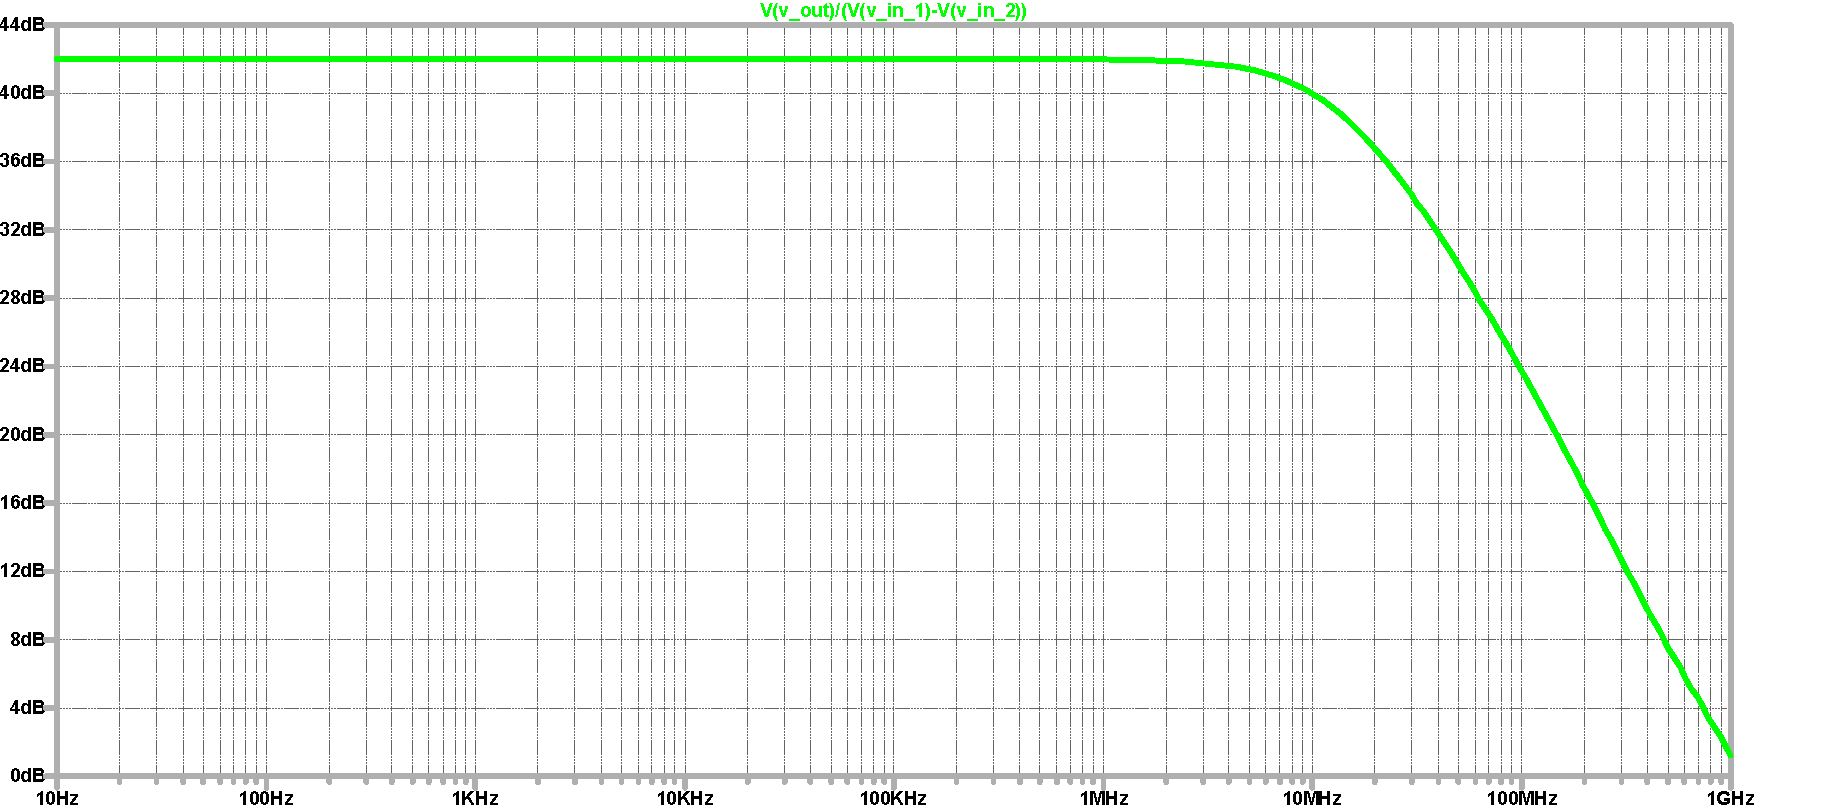
\includegraphics[width=.9\linewidth]{img/q3/dm.pdf}
\caption{\label{fig:dm-q3}Differential gain of differential pair}
\end{figure}

\item Common mode gain

From figure \ref{fig:cm-q3}, \(A_{CM} = -48.4 dB\)
\begin{figure}[H]
\centering
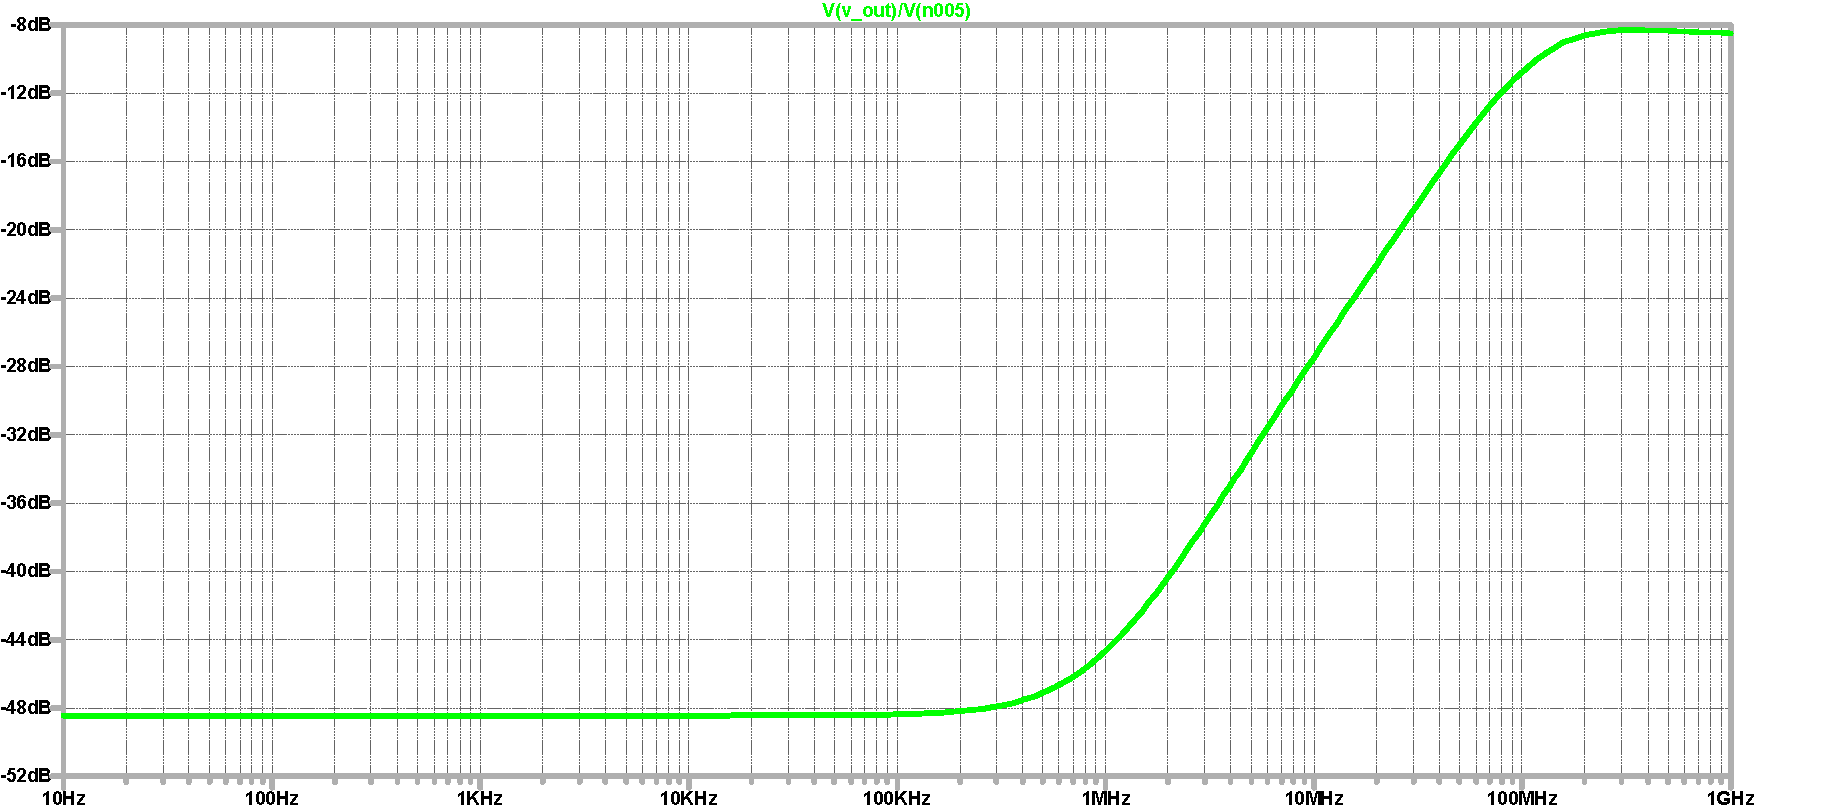
\includegraphics[width=.9\linewidth]{img/q3/cm.pdf}
\caption{\label{fig:cm-q3}Common mode gain of differential pair}
\end{figure}
\end{enumerate}
\end{enumerate}

\section{Problem 4}
\label{sec:orgdf12f4f}
The final circuit NMOS differential pair with PMOS current mirror load and cascode stages are shown in figure \ref{fig:diff-mirror-cascode-q4}.
\begin{figure}[H]
\centering
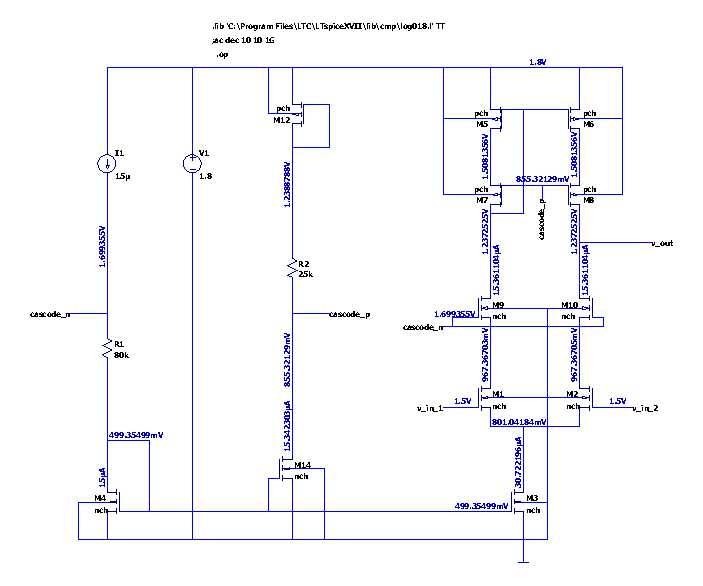
\includegraphics[width=.9\linewidth]{img/q4/diff-mirror-cascode-1.pdf}
\caption{\label{fig:diff-mirror-cascode-q4}Bias points for NMOS differential pair with PMOS current mirror load and cascode stage}
\end{figure}

The following images show the device operating points.
\begin{figure}[H]
\centering
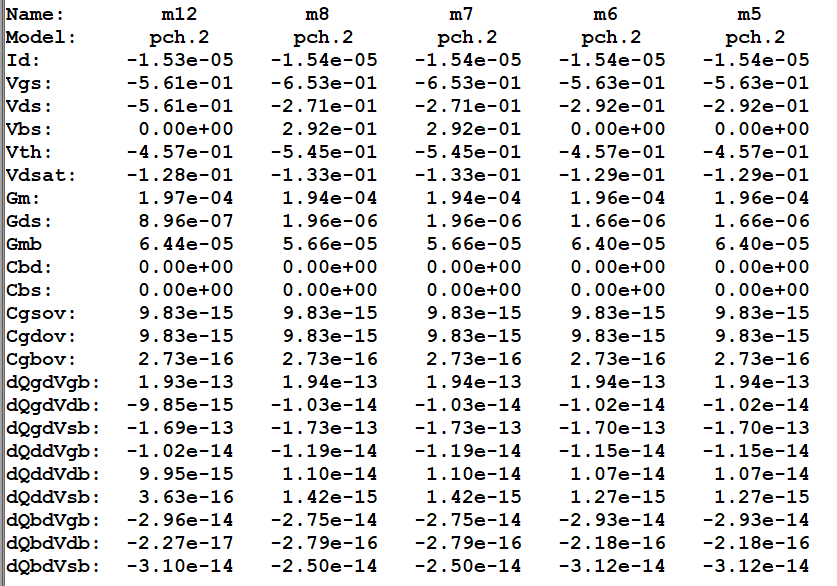
\includegraphics[height=300px]{img/q4/error-log/error-log-1.png}
\caption{\label{fig:err-1-q4}Spice error log file 1}
\end{figure}

\begin{figure}[H]
\centering
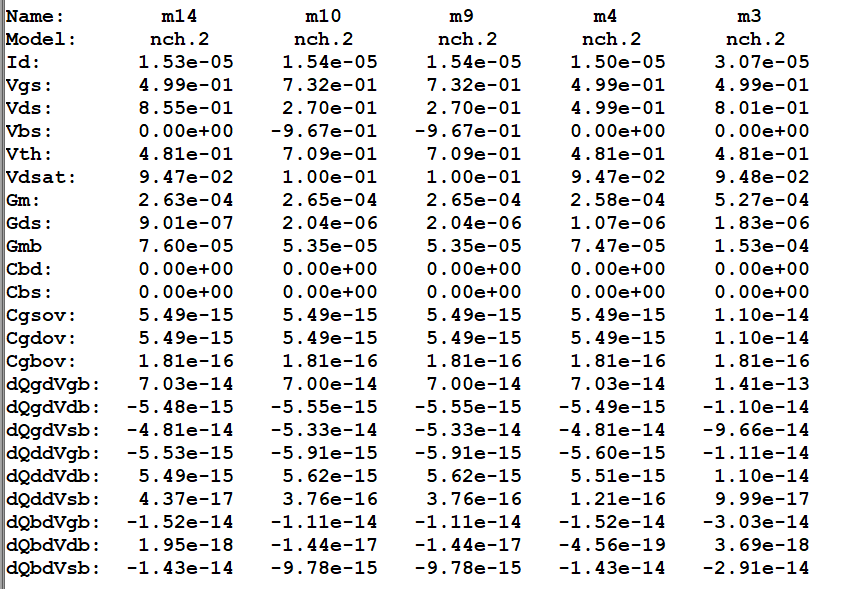
\includegraphics[height=300px]{img/q4/error-log/error-log-2.png}
\caption{\label{fig:err-2-q4}Spice error log file 2}
\end{figure}

\begin{figure}[H]
\centering
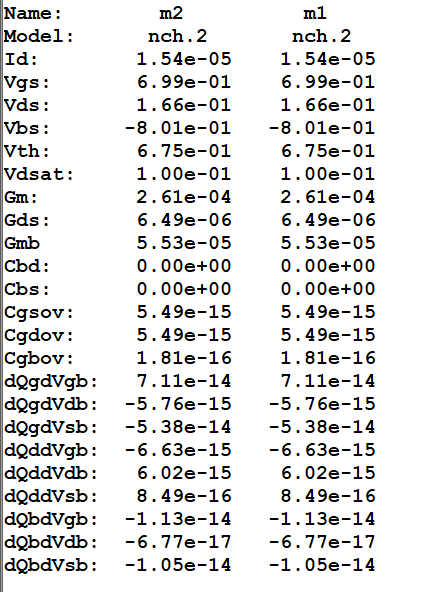
\includegraphics[height=300px]{img/q4/error-log/error-log-3.png}
\caption{\label{fig:err-3-q4}Spice error log file 3}
\end{figure}

The following sections roughly estimates the bias points for saturation.
\begin{enumerate}[(a)]
\item For biasing V\textsubscript{cascode\textsubscript{n}}, the staturation conditions for each transistor starting from the ground.
\begin{enumerate}[1.]
\item M3
\begin{equation*}
\begin{aligned}
V_{D3} &\geq V_{G3} - V_{TH3} \\
\end{aligned}
\end{equation*}
\item M1
\begin{equation*}
\begin{aligned}
V_{D1} - V_{S1} &\geq V_{G1} - V_{S1} - V_{TH1} \\
V_{D1} &\geq V_{G1} - V_{TH1} \\
V_{D1} &\geq 1.5V - 0.675V \\
V_{D1} &\geq 0.825V
\end{aligned}
\end{equation*}
\item M9
\begin{equation*}
\begin{aligned}
V_{D9} - V_{S9} &\geq V_{G9} - V_{S9} - V_{TH9} \\
V_{D9} &\geq V_{G9} - V_{TH9} \\
V_{G9} &\leq V_{D9} + V_{TH9} \\
\\
V_{G9} - V_{S9} &\geq V_{TH9} \\
V_{G9} &\geq 0.825V + 0.709V \\
V_{G9} &\geq 1.534V \\
\end{aligned}
\end{equation*}
\end{enumerate}
\end{enumerate}


Since only one current source is available and using a NMOS current mirror PMOS diode connected current source will not be able to
acheive voltage of 1.534V (> V\textsubscript{DD} - V\textsubscript{THp}), the remaining option is to attach a resistor to the
current source circuit line.

The required resistance,
\begin{equation*}
\begin{aligned}
R &\geq \frac{1.5V - V_{D4}}{15\mu{}A} \\
&\geq 68.93k \Omega \\
\end{aligned}
\end{equation*}
In the simulation, the resistance is increased to 80k to increase the DM gain.


\begin{enumerate}
\item For biasing V\textsubscript{cascode\textsubscript{p}}, a maximum voltage for keeping the circuit in saturation is desired
for maximizing the voltage swing. The saturation for transistor starting from V\textsubscript{DD}.
\begin{enumerate}
\item M5
Maximum value of V\textsubscript{D}
\begin{equation*}
\begin{aligned}
Max(V_{D}) &= V_{DD} - |V_{TH5}| \\
&= 1.8V - 0.457V \\
&= 1.343V \\
\end{aligned}
\end{equation*}
\item M7
\begin{equation*}
\begin{aligned}
V_{S7} - V_{G7} &\geq V_{TH7} \\
V_{G7} &\leq 1.343V - 0.543V \\
V_{G7} &\leq 0.8V \\
\end{aligned}
\end{equation*}
\end{enumerate}
\end{enumerate}


In this case using a NMOS current mirror PMOS diode connected current source is possible for bias voltage of
0.8V (< V\textsubscript{DD} - V\textsubscript{THp}).

The required resistance,
\begin{equation*}
\begin{aligned}
R &= \frac{1.8V - V_{TH12} - V_{D4}}{15\mu{}A} \\
&= 27.376k \Omega \\
\end{aligned}
\end{equation*}

Similar to the previous section, the resistance in the simulation is decreased to increase the DM gain.
\section{Problem 5}
\label{sec:org8862ed4}
\begin{enumerate}[(a)]
\item Differential gain

From figure \ref{fig:dm-q5}, \(A_{DM} = 73.6 dB\)
\begin{figure}[H]
\centering
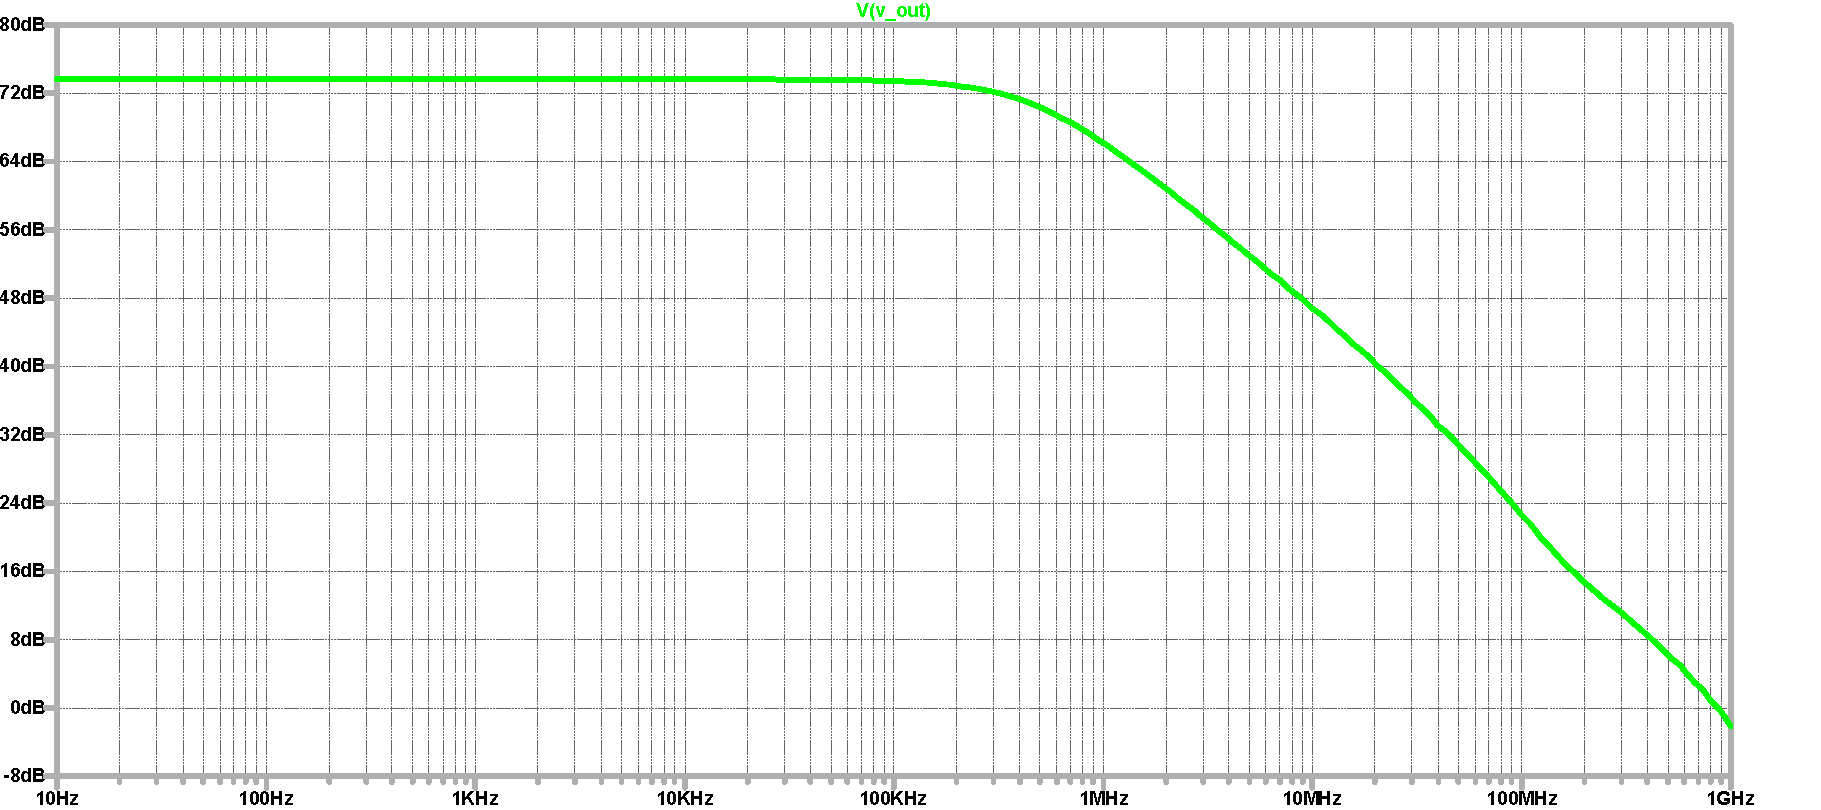
\includegraphics[width=.9\linewidth]{img/q5/dm.pdf}
\caption{\label{fig:dm-q5}Differential gain of differential pair}
\end{figure}
\item Common-mode gain

From figure \ref{fig:cm-q5}, \(A_{CM} = -48.4 dB\)
\begin{figure}[H]
\centering
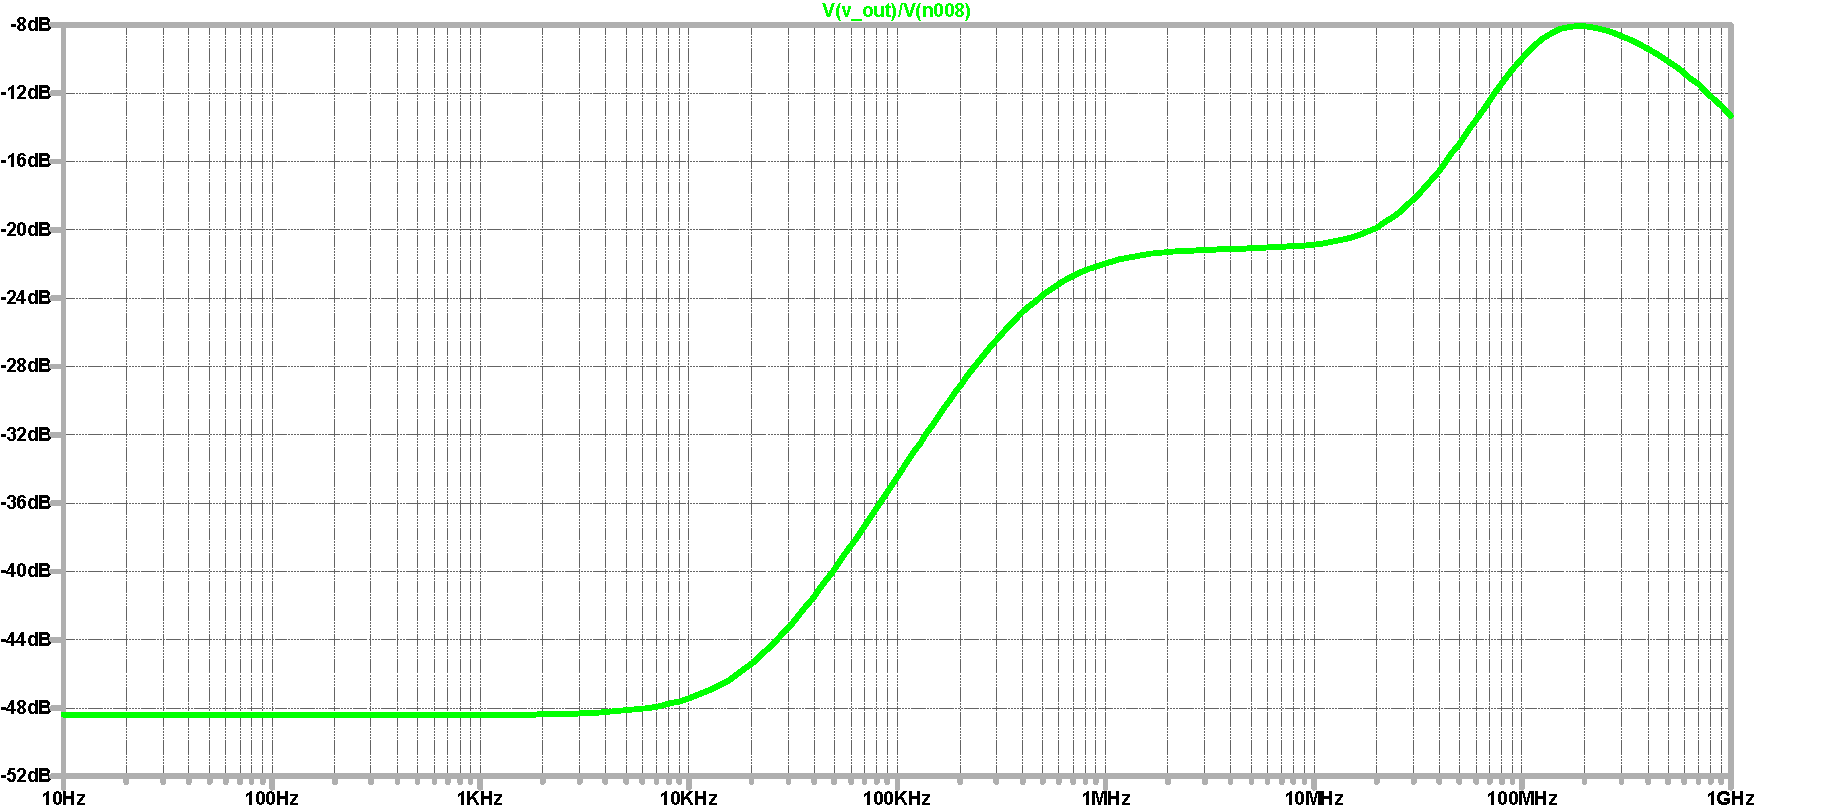
\includegraphics[width=.9\linewidth]{img/q5/cm.pdf}
\caption{\label{fig:cm-q5}Common mode gain of differential pair}
\end{figure}
\end{enumerate}
\end{document}
